\documentclass[../../../../main.tex]{subfiles}
\begin{document}

\begin{flushright}
\footnotesize\textit{【自動文字起こし・要確認】}
\end{flushright}

[解]\\
(1) $C(0, -1, \sqrt{2}), D(0, 1, \sqrt{2})$\\
とすると四面体ABCDは\\
一辺2の正四面体となり\\
題意をみたす。

\begin{center}
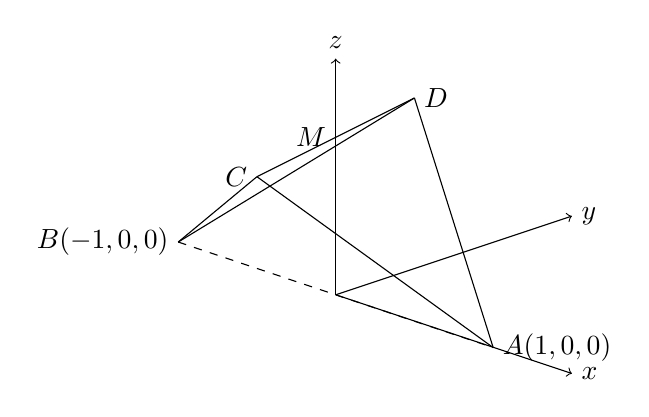
\begin{tikzpicture}[scale=1]
    \draw[->] (0,0) -- (3, -1) node[right] {$x$};
    \draw[->] (0,0) -- (3, 1) node[right] {$y$};
    \draw[->] (0,0) -- (0, 3) node[above] {$z$};
    \coordinate (O) at (0,0);
    \coordinate (A) at (2, -0.67);
    \coordinate (B) at (-2, 0.67);
    \coordinate (M) at (0, 2);
    \coordinate (C) at (-1, 1.5);
    \coordinate (D) at (1, 2.5);
    \draw[dashed] (B) -- (O) -- (A);
    \node[right] at (A) {$A(1,0,0)$};
    \node[left] at (B) {$B(-1,0,0)$};
    \node[left] at (C) {$C$};
    \node[right] at (D) {$D$};
    \node[left] at (M) {$M$};
    \draw (C) -- (D);
    \draw (A) -- (C);
    \draw (A) -- (D);
    \draw (B) -- (C);
    \draw (B) -- (D);
\end{tikzpicture}
\end{center}

(2) $\alpha$とz軸の交点$H$は$OM=\sqrt{2}$から$H(0, 0, t\sqrt{2})$である。\\
$\alpha$で切断すると、切り口はz軸に\\
垂直な四角形になり右の切断図から、\\
下図のようになる

\begin{center}
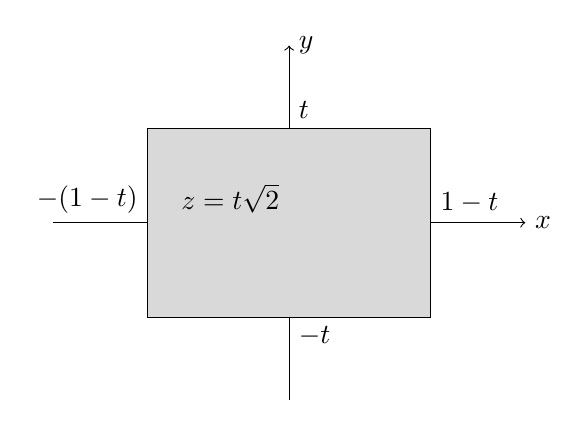
\begin{tikzpicture}[scale=1.5]
    \draw[->] (-2,0) -- (2,0) node[right] {$x$};
    \draw[->] (0,-1.5) -- (0,1.5) node[right] {$y$};
    \draw[fill=gray!30] (-1.2, -0.8) rectangle (1.2, 0.8);
    \node[above right] at (0, 0.8) {$t$};
    \node[below right] at (0, -0.8) {$-t$};
    \node[above right] at (1.2, 0) {$1-t$};
    \node[above left] at (-1.2, 0) {$-(1-t)$};
    \node[above left] at (0,0) {$z=t\sqrt{2}$};
\end{tikzpicture}
\hspace{1cm}
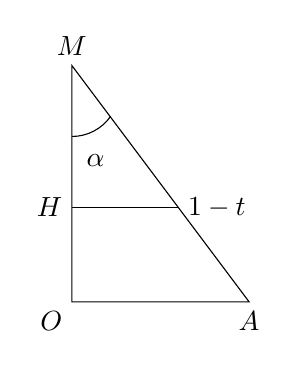
\begin{tikzpicture}[scale=1.5]
    \coordinate (M) at (0, 2);
    \coordinate (O) at (0, 0);
    \coordinate (A) at (1.5, 0);
    \coordinate (H) at (0, 0.8);
    \coordinate (P) at (0.9, 0.8);
    \draw (M) node[above] {$M$} -- (O) node[below left] {$O$} -- (A) node[below] {$A$} -- cycle;
    \draw (H) node[left] {$H$} -- (P);
    \node[right] at (P) {$1-t$};
    \draw (0, 1.4) arc (270:325:0.4);
    \node at (0.2, 1.2) {$\alpha$};
\end{tikzpicture}
\hspace{1cm}
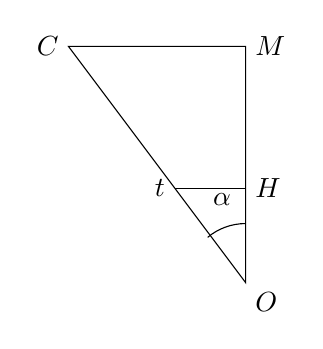
\begin{tikzpicture}[scale=1.5]
    \coordinate (C) at (-1.5, 2);
    \coordinate (M) at (0, 2);
    \coordinate (O) at (0, 0);
    \coordinate (H) at (0, 0.8);
    \coordinate (Q) at (-0.6, 0.8);
    \draw (C) node[left] {$C$} -- (M) node[right] {$M$} -- (O) node[below right] {$O$} -- cycle;
    \draw (H) node[right] {$H$} -- (Q);
    \node[left] at (Q) {$t$};
    \draw (0, 0.5) arc (90:130:0.5);
    \node at (-0.2, 0.7) {$\alpha$};
\end{tikzpicture}
\end{center}

(3) (2)と同じくして$z=k\sqrt{2}$における切り口の面積$S(k)$は（$0 \le k \le t$）
\[ S(k) = 2(1-k) \cdot 2k = 4k(1-k) \]
だから、求める体積$V$は
\begin{align*}
V &= \int_0^{t\sqrt{2}} S(k) dz \\
&= \int_0^t S(k) \frac{dz}{dk} dk \\
&= \int_0^t 4k(1-k) \sqrt{2} dk \\
&= 4\sqrt{2} \left[ \frac{1}{2}k^2 - \frac{1}{3}k^3 \right]_0^t \\
&= 4\sqrt{2} \left( \frac{1}{2}t^2 - \frac{1}{3}t^3 \right) \quad //
\end{align*}

{\color{cyan}
[本時のミス]\\
$\circ$ 1文字の代入ミス $\Rightarrow$ 検算でひっかからない系\\
$\Rightarrow$ {\color{orange} 1行戻りの大切さ}\\
$\circ$ また座標まちがえた\dots
}

\end{document}
